% unicodeは、hyperrefへの指定で、pdfのメタデータにあるタイトルの文字化けを防ぐ
% ptは細かい指定はできないらしい
% チートシート
% https://www.cpt.univ-mrs.fr/~masson/latex/Beamer-appearance-cheat-sheet.pdf
\documentclass[unicode, 14pt, aspectratio=169]{beamer}
% \usepackage{listings}
% \usepackage{enumitem}
% \usepackage{xcolor}
% \usepackage{textcomp}
\usetheme{titech}
\addbibresource{main.bib}
 \date{\number\year 年\number\month 月\number\day 日}
\title{型理論のはじまり}
\author{\texttt{ryotaro612}} 
\begin{document}
\newcommand\blfootnote[1]{
    \begingroup
    \renewcommand\thefootnote{}\footnote{#1}
    \addtocounter{footnote}{-1}
    \endgroup
}

\begin{frame}[noframenumbering, plain]
\titlepage
\end{frame}
\section{導入}
\begin{frame}
  \frametitle{資料の目的}
  {\large 型理論の関連分野に興味もってもらう}
  \par
  \vspace{16pt}
  参考資料が関係する分野
  \begin{itemize}
  \item 論理学
  \item 集合論
  \item 記号論
  \item 構造主義
  \item 哲学、とくに分析哲学
  \end{itemize}
\end{frame}
\section{非ユークリッド幾何学の発見}
  % タレス、ピタゴラス、プラトンアカデメイア、アリストテレス
  % アルキメデス 有理数
  % 球体
  % ロバチェフスキー
  % 公準
  % 素朴集合論
  % 双曲平面橋爪
\begin{frame}
  \frametitle{ギリシアで発展した幾何学}
  {\large 幾何学の知識は証明された定理の集積}
\begin{columns}
  \begin{column}{0.25\textwidth}  %%<--- here
    \begin{center}
      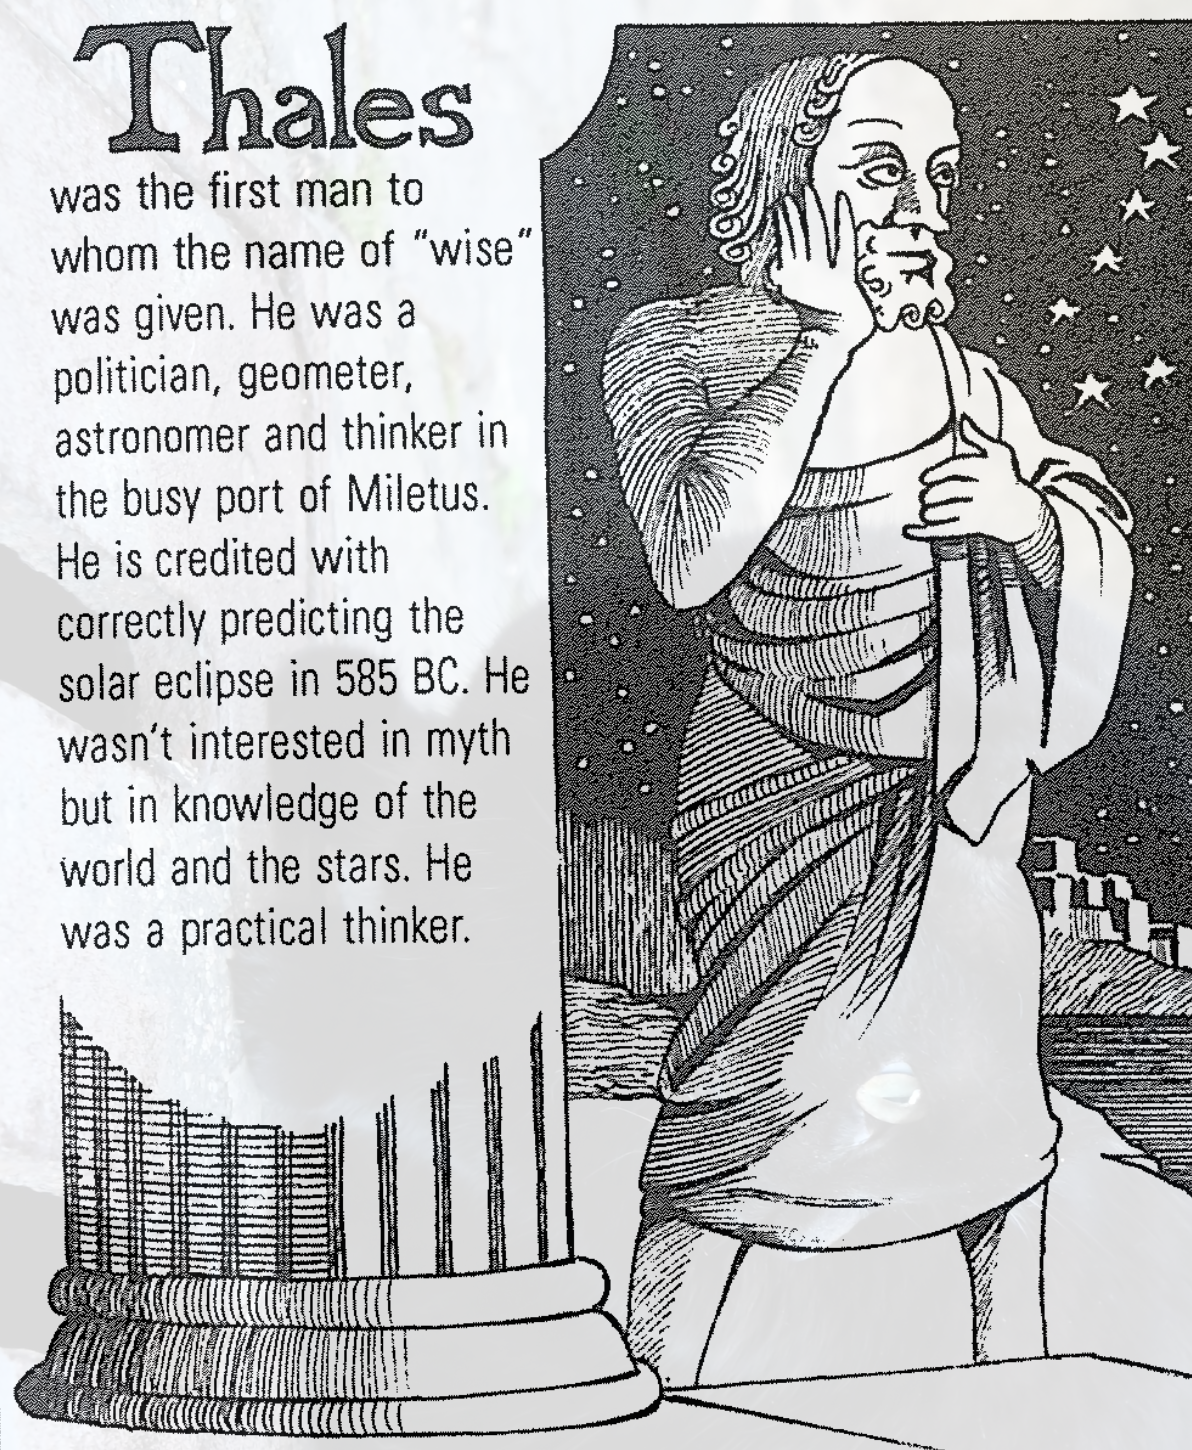
\includegraphics[width=0.8\textwidth]{images/thales.png}
    \end{center}
  \end{column}
  \begin{column}{0.25\textwidth}  %%<--- here
    \begin{center}
      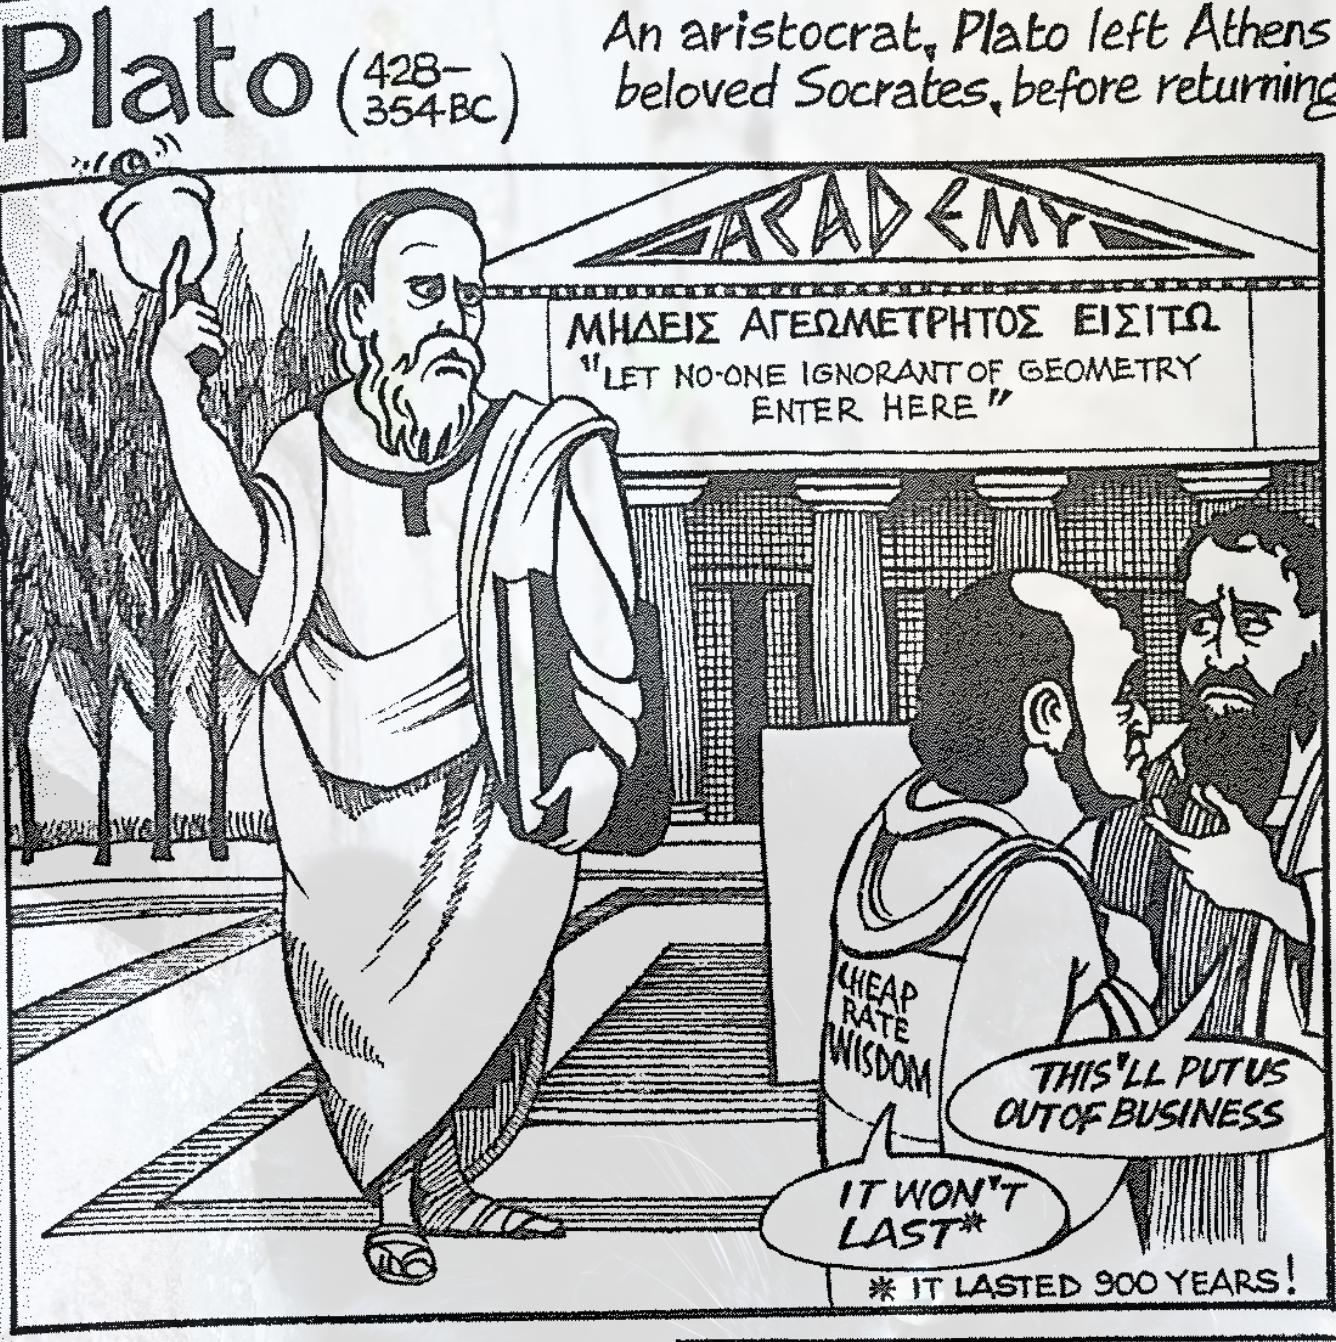
\includegraphics[width=0.8\textwidth]{images/plato.png}
    \end{center}
  \end{column}
  \begin{column}{0.25\textwidth}  %%<--- here
    \begin{center}
      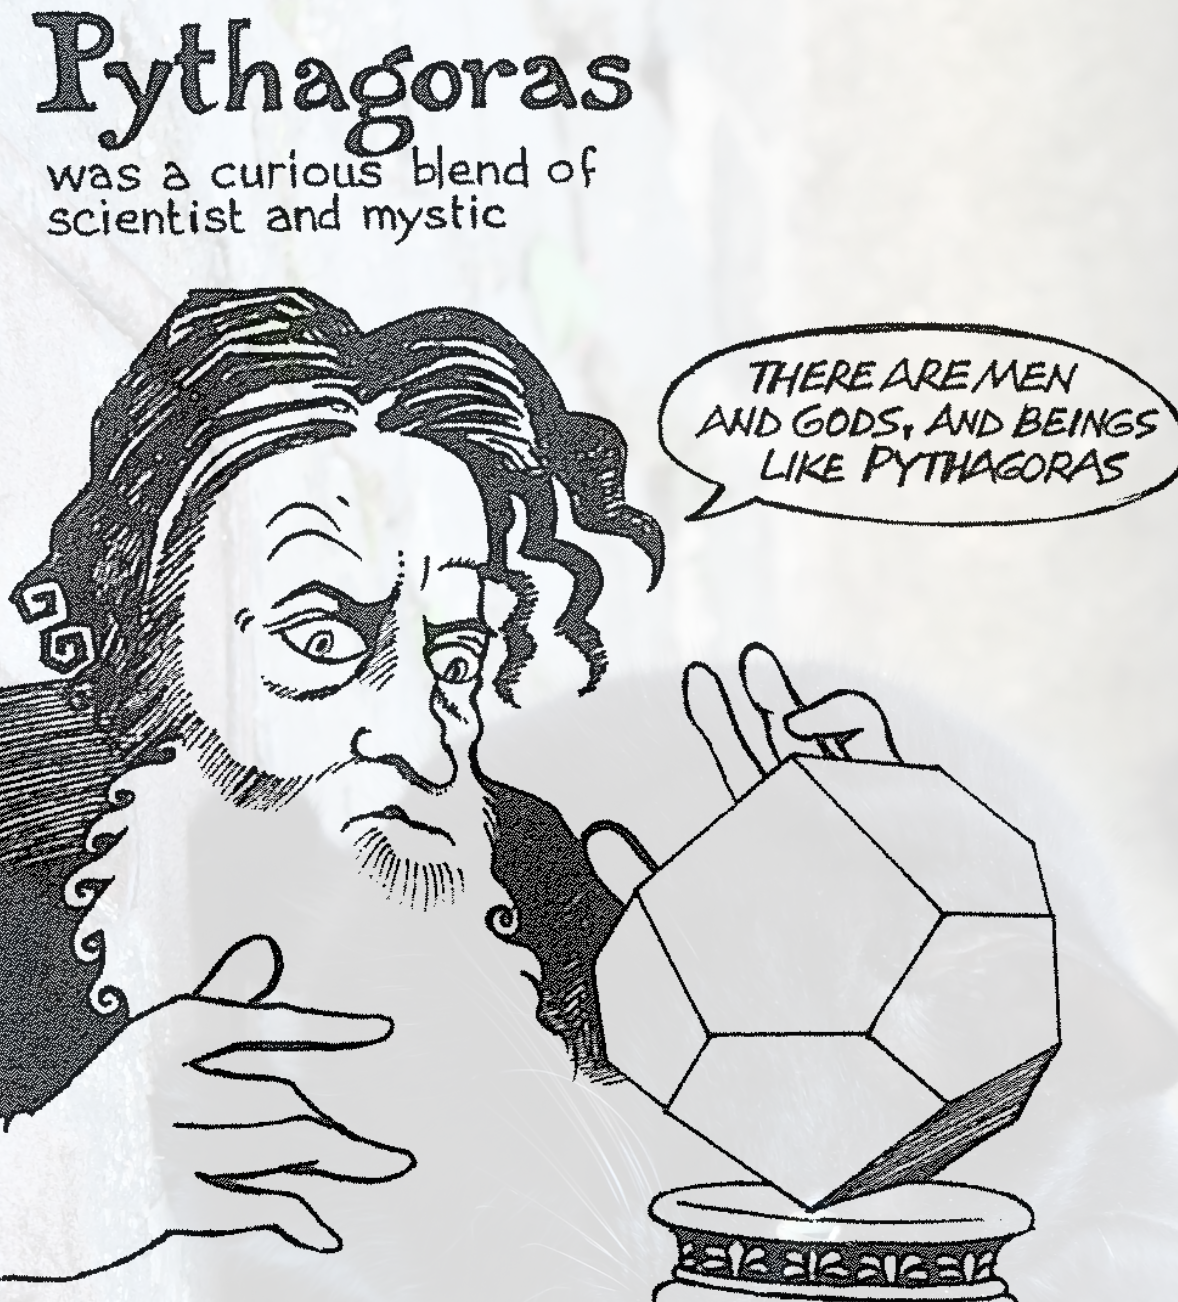
\includegraphics[width=0.8\textwidth]{images/pythagoras.png}
    \end{center}
  \end{column}
  \begin{column}{0.25\textwidth}  %%<--- here
    \begin{center}
      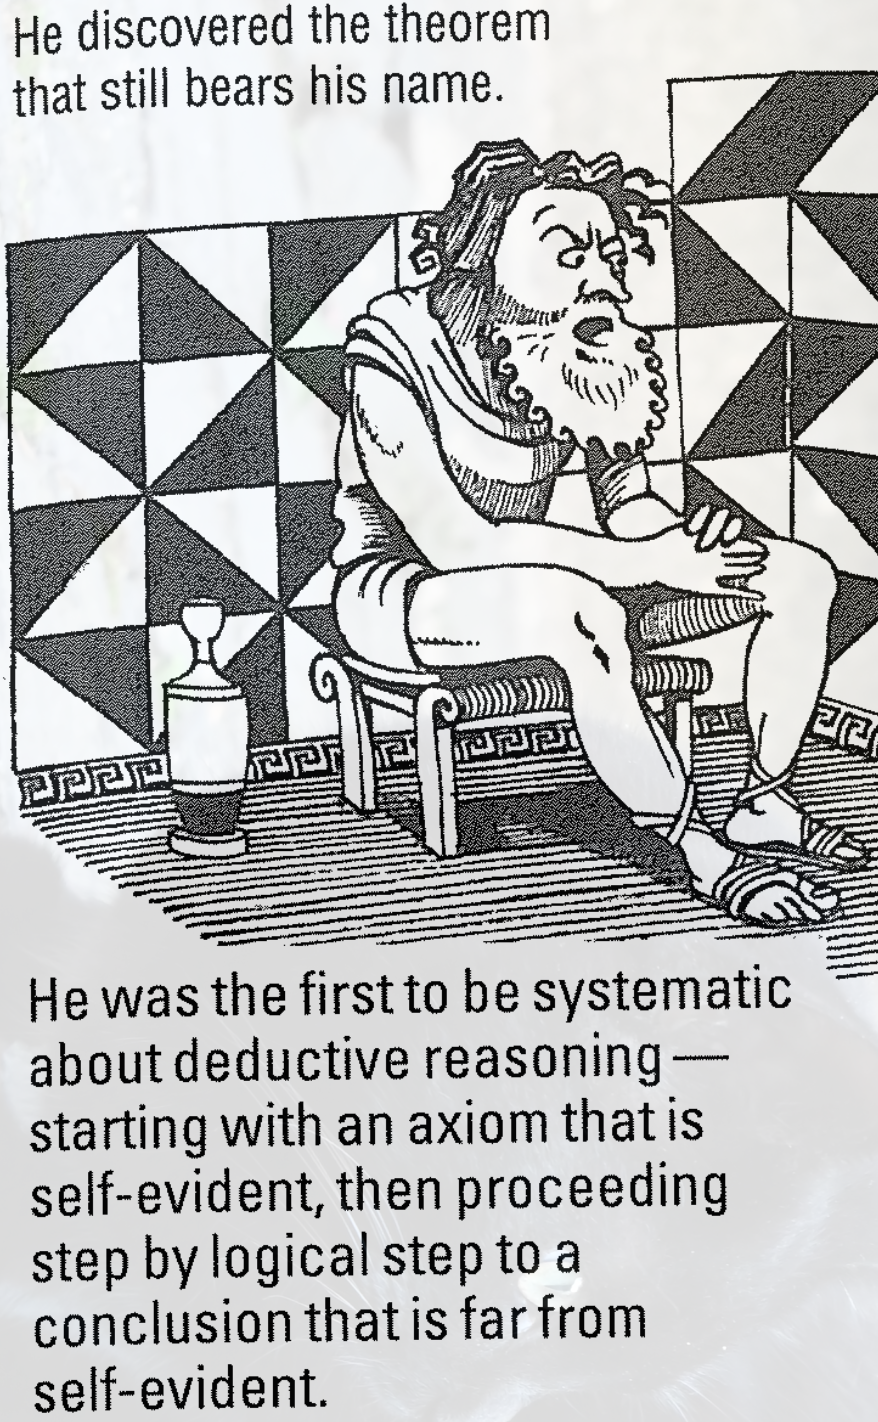
\includegraphics[width=0.8\textwidth]{images/pythagoras2.png}
    \end{center}
  \end{column}  
\end{columns}
\blfootnote{図はPhilosophy for beginners\supercite{philosophy-for-begginers}より} 
\end{frame}
\begin{frame}
  \frametitle{ユークリッドの原論}
  {\large 幾何学が定義、公理、公準、命題、証明に整理された}
  \par
  \vspace{16pt}
  具体例
  \begin{description}
  \item[定義1] 点とは部分をもたないもの
  \item[定義2] 線は幅のない長さ
  \item[定義3] 面は長さと幅だけをもつもの
  \item[公理5] 全体は部分より大きい
  \item[命題5] 二等辺三角形の底辺はたがいに等しい
  \end{description}
  % ユークリッドはギリシア数学の知識を5つの公準から
\end{frame}
\begin{frame}
  \frametitle{5つの公準}
  {\large 5番目の平行線の公準は複雑}
  \par
  \vspace{16pt}  
  \begin{enumerate}
  \item 任意の点から任意の点に直線を引くこと
  \item 有限な線分を連続して直線に延長すること
  \item 任意の点と半径で円を描くこと
  \item すべての直角は等しいこと
  \item 二直線が一直線と交わるとき、同じ側にできる内角の和が\\二直角よりも小さいなら二直線はその側に延長すると交わる
  \end{enumerate}
\end{frame}
\begin{frame}[t]
  \frametitle{公準5の別名は平行線公理}
  {\large 任意の直線と直線外の任意の一点があるとき\\一点を通り直線に平行な直線は1本だけ}
  \blfootnote{図は『数学の世界史』\supercite{suugaku-no-sekaishi}より}
  \begin{figure}
    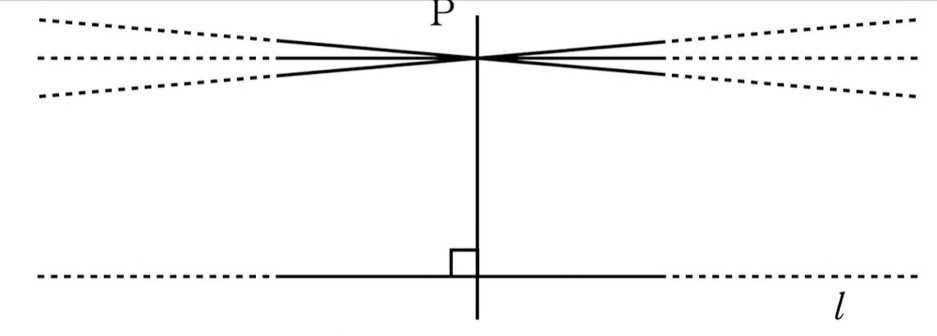
\includegraphics[width=0.7\textwidth]{images/axiom5.png}
    \caption{平行線と直線}
  \end{figure}
\end{frame}
\begin{frame}
  \frametitle{平行線公理への疑問}
  {\large 平行線公理をほかの公準から証明できるか}
  \begin{itemize}
  \item ほかの公準からの証明を試みる
    \begin{itemize}
    \item アラビア世界ではハイタム(965-1039)やハイヤーミー(1048 – 1131)
    \item サッケーリ(1667ー1733), ルシャンドル(1752-1833)は独立に\\
      平行線公理がないと三角形の内角の和は二直角以下になると証明
    \end{itemize}
  \item 平行線公理を否定しても、ほかの公準と矛盾しない
    \begin{itemize}
    \item ガウス(1777-1855)は平行線の公理は証明できないことを示唆する手紙を残す
    \item ロバチェフスキー(1792-1856)とボヤイ(1802-1860)が独立に平行線を二本以上ひけても矛盾しない非ユークリッド幾何学を発見
    \end{itemize}
  \end{itemize}
  % たんなる仮説なのか
  % ほかの公準から導出できるか
% 直線$l$上にない任意の点$P$を通る直線$l$の平行線は2本以上ある
\end{frame}
\begin{frame}
  \frametitle{例 球面幾何学の平行線}
  {\large 測地線があたえられるとき、その測地線にない点pをとおり測地線と交わらない測地線はない}
  たんなる仮説なのか
  ほかの公準から導出できるか
\end{frame}
\begin{frame}
  \frametitle{非ユークリッド幾何学の発見の影響}
  {\large 「正しさ」は仮定した公理から作りだすもの}
\end{frame}
\section{素朴な集合論と記号論理学}
\begin{frame}
  \frametitle{ものの集まりで数学を考える}
  {\large いろんな数学の概念を集合で定義できる}
\end{frame}
\begin{frame}
  \frametitle{算術の基礎}
  {\large フレーゲは記号論理学と集合論による自然数の公理と定理の提供を試みた}
\end{frame}
\begin{frame}
  \frametitle{思考を計算するための記号}
  {\large 推論の規則を記号を操作する計算に還元する考えは世紀以前からある}
\end{frame}
\begin{frame}
  \frametitle{ブールの論理代数}
  {\large ブールは命題に出現する個体の集合を記号で表した}
  % https://archive.org/stream/THELAWSOFTHOUGHTGeorgeBoole/THE%20LAWS%20OF%20THOUGHT_George%20Boole_djvu.txt
\end{frame}
\begin{frame}
  \frametitle{推論規則の例}
  {\large 命題論理は、命題と論理結合子からなる論理体系}
\end{frame}
\begin{frame}
  \frametitle{概念記法}
  {\large フレーゲは述語の言明を形式化した}
\end{frame}
\begin{frame}
  \frametitle{ラッセルのパラドクス}
  {\large 集合の集合を考えると矛盾がおきる}
\end{frame}
\begin{frame}
  \frametitle{型の概念}
  ラッセルの自分自身に言明する述語の例に対して、フレーゲは述語は述語を引数にとれないと回答した

  ただし述語の外延が作用する
\end{frame}
% https://fair-use.org/bertrand-russell/the-principles-of-mathematics/s498
% https://plato.stanford.edu/entries/type-theory/
% https://people.umass.edu/klement/pom/pom-portrait.pdf
% https://repository.kulib.kyoto-u.ac.jp/dspace/bitstream/2433/151121/1/ronso38_S49_type.pdf
% https://www.britannica.com/topic/theory-of-types-logic
\begin{frame}[allowframebreaks,t]
  \frametitle{参考資料}
  \printbibliography
  \nocite{*}
\end{frame}

\end{document}
